\documentclass[tikz,border=6pt]{standalone}
\usepackage{helvet}
\usetikzlibrary{arrows.meta}
\definecolor{ri}{HTML}{DAE8FC}
\definecolor{riborder}{HTML}{7C9AC4}
\definecolor{rpa}{HTML}{D5E8D4}
\definecolor{rpaborder}{HTML}{82B366}
\definecolor{data}{HTML}{57920D}
\definecolor{exchange}{HTML}{FFE6CC}
\definecolor{correlation}{HTML}{F8CECC}
\definecolor{total}{HTML}{E1D5E7}
\definecolor{exborder}{HTML}{D6A000}
\definecolor{ecborder}{HTML}{B85450}
\definecolor{totalborder}{HTML}{9673A6}
\begin{document}
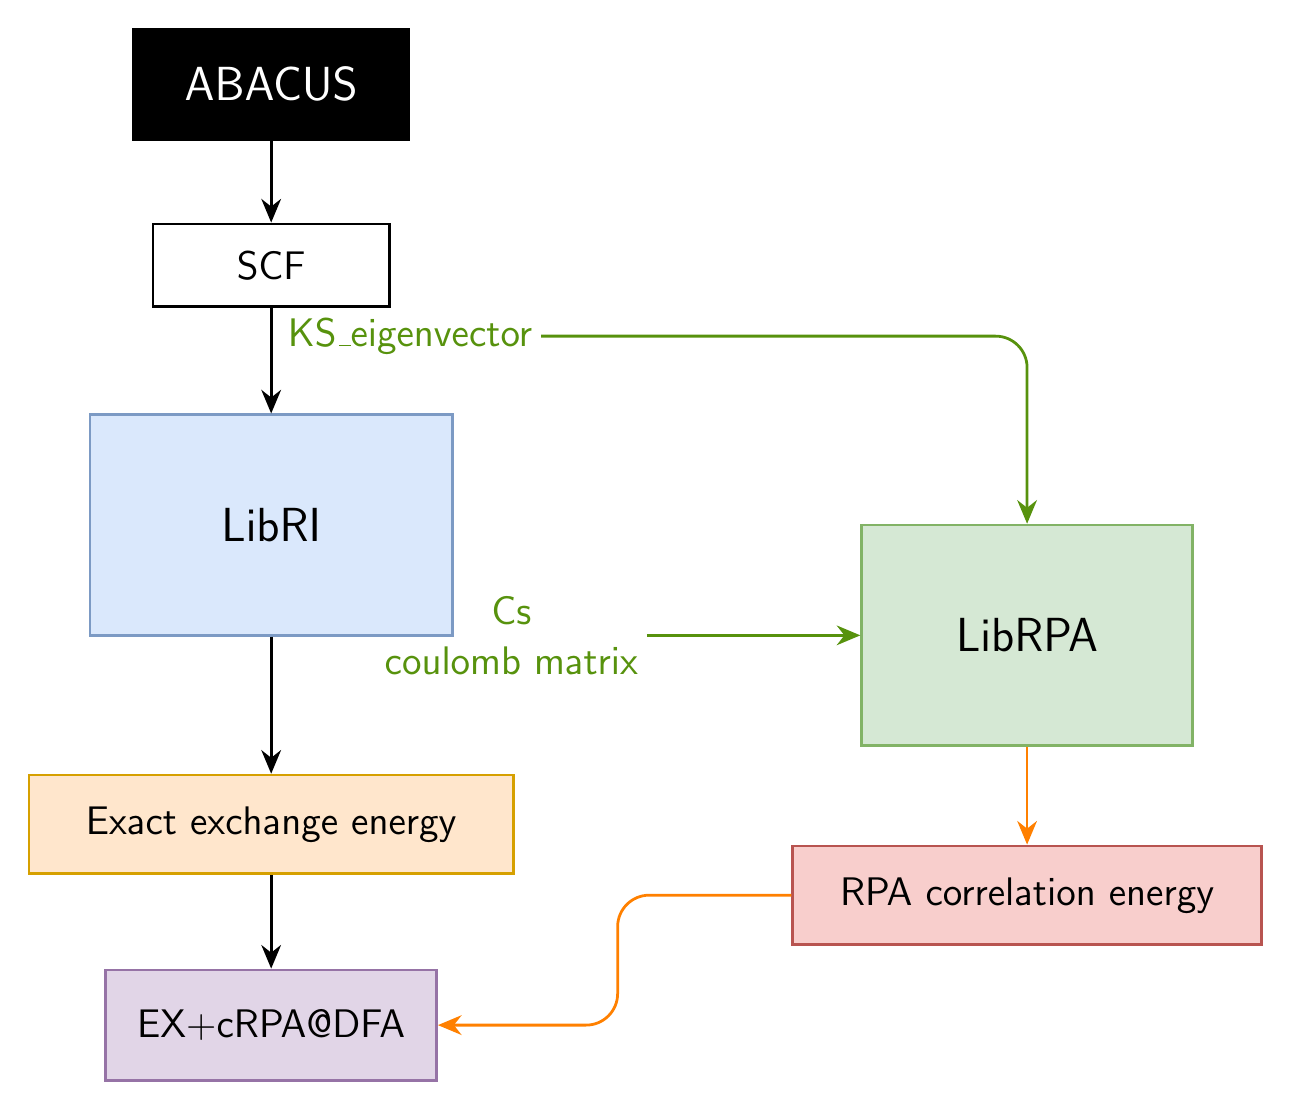
\begin{tikzpicture}[
  font=\sffamily\Large,
  box/.style={draw=black,line width=1pt,fill=white,align=center,
    inner sep=6pt},
  arrow/.style={-{Stealth[length=3mm,width=2.5mm]},line width=1pt},
  datalabel/.style={text=data,align=center,inner sep=3pt}]

\node[box,fill=black,text=white,minimum width=3.5cm,minimum height=1.4cm,
  font=\sffamily\LARGE] (abacus) at (3.5,12.5) {ABACUS};
\node[box,minimum width=3cm,minimum height=1.05cm] (scf) at (3.5,10.2) {SCF};
\node[box,fill=ri,draw=riborder,minimum width=4.6cm,minimum height=2.8cm,
  font=\sffamily\LARGE] (libri) at (3.5,6.9) {LibRI};
\node[box,fill=exchange,draw=exborder,minimum width=6.15cm,
  minimum height=1.25cm] (exx) at (3.5,3.1) {Exact exchange energy};
\node[box,fill=total,draw=totalborder,minimum width=4.2cm,minimum height=1.4cm]
  (out) at (3.5,.55) {EX+cRPA@DFA};
\draw[arrow] (abacus) -- (scf);
\draw[arrow] (scf) -- (libri);
\draw[arrow] (libri) -- (exx);
\draw[arrow] (exx) -- (out);

\node[box,fill=rpa,draw=rpaborder,minimum width=4.2cm,minimum height=2.8cm,
  font=\sffamily\LARGE] (librpa) at (13.1,5.5) {LibRPA};
\node[box,fill=correlation,draw=ecborder,minimum width=5.95cm,
  minimum height=1.25cm] (ec) at (13.1,2.2) {RPA correlation energy};
\draw[arrow,orange] (librpa) -- (ec);
\draw[arrow,orange,rounded corners=4mm]
  (ec.west) -- (7.9,2.2) -- (7.9,.55) -- (out.east);

\node[datalabel,anchor=west] (ks) at (3.6,9.3) {KS\_eigenvector};
\draw[arrow,data,rounded corners=4mm]
  (ks.east) -- (13.1,9.3) -- (librpa.north);
\node[datalabel] (cs) at (6.55,5.5) {Cs\\coulomb matrix};
\draw[arrow,data] (cs.east) -- (librpa.west);
\end{tikzpicture}
\end{document}
